% Author: Izaak Neutelings (July 2023)
% Description:
%   Standard Model (SM) of Particles Physics table (round)
% Inspired by:
%   https://www.symmetrymagazine.org/article/july-2015/standard-model?language_content_entity=und
%   https://www.quantamagazine.org/a-new-map-of-the-standard-model-of-particle-physics-20201022/
%   https://www.energy.gov/science/doe-explainsthe-standard-model-particle-physics
\documentclass[border=3pt,tikz]{standalone}
\usepackage{amsmath} % for \text
\usepackage{xfrac} % for \myfrac
\usepackage{bm} % for \bm
\usetikzlibrary{calc}
\usetikzlibrary{positioning}
\tikzset{>=latex} % for LaTeX arrow head

% FONT
\usepackage{sansmath} % for \sansmath
\renewcommand{\familydefault}{\sfdefault} % set sans serif font globally
\sansmath % set sans serif font globally

% UNSLANT GREEK LETTERS for particle symbols
% https://tex.stackexchange.com/questions/145926/upright-greek-font-fitting-to-computer-modern
% https://tex.stackexchange.com/questions/236915/adjust-custom-made-upright-greek-letters-when-used-in-subscripts
\usepackage{scalerel}
\newsavebox{\foobox}
\newcommand{\slantbox}[2][0]{\mbox{%
  \sbox{\foobox}{#2}%
  \hskip\wd\foobox
  \pdfsave
  \pdfsetmatrix{1 0 #1 1}%
  \llap{\usebox{\foobox}}%
  \pdfrestore
}}
\newcommand\unslant[2][-.25]{%
  %\mkern1.2mu%
  \ThisStyle{\slantbox[#1]{$\SavedStyle#2$}}%
  \mkern-2.2mu%
}
\newcommand\PGm{\unslant\mu} % muon
\newcommand\PGt{\unslant\tau} % tau
\newcommand\PGn[1]{\unslant\nu_{#1}\mkern-1.5mu} % neutrino
\newcommand\PSGn[1]{\widetilde{\unslant\nu}_{\mathrm{#1}}\mkern-1.5mu} % sneutrino
\newcommand\mytilde[1]{\widetilde{\mathrm{#1}}} % tilde with math roman

% COLORS
\colorlet{mylightblue}{blue!60!cyan!80!black!15}
\colorlet{mypurple}{blue!50!red!70}
\colorlet{gaugecol}{red!90!black!70} % Wiki red
\colorlet{leptoncol}{green!80!black!70} % Wiki green
\colorlet{quarkcol}{blue!85!cyan!95!black!55} % Wiki purple
\colorlet{scalarcol}{yellow!70!orange!98!black}

% STYLES
\tikzstyle{particle}=[black,thick,align=center]
\tikzstyle{lepton}=[particle,fill=leptoncol!#1] %,inline=leptoncol!#1]
\tikzstyle{quark}=[particle,fill=quarkcol!#1] %,inline=quarkcol!#1]
\tikzstyle{gauge}=[particle,fill=gaugecol!#1] %,inline=gaugecol!#1]
\tikzstyle{scalar}=[particle,fill=scalarcol!#1] %,inline=scalarcol!#1]

%%%% INTERNAL LINES
%%%\newlength{\internalborderwidth}
%%%\setlength{\internalborderwidth}{2pt}
%%%\tikzset{
%%%  inline/.style={
%%%    postaction={clip,postaction={draw=#1!white!80!black,solid,line width=\internalborderwidth},
%%%                postaction={draw}}
%%%}}

% MACROS
\def\Rhiggs{0.37} % outer radius of Higgs boson layer
\def\Rboson{1.1}  % outer radius of gauge boson layer
\def\Rfermion{2}  % outer radius of fermion layer
\def\higgs{
  \draw[scalar] (O) circle(\Rhiggs);
  %\node[fill=none] at (O) {H};
  \coordinate (H) at (O);
}
\def\boson[#1]#2{
  %\draw[#1] (O) -- (#2:\Rboson) arc(#2:#2+90:\Rboson) -- cycle;
  \draw[#1] (#2:\Rhiggs) -- (#2:\Rboson) arc(#2:#2+90:\Rboson)
    -- (#2+90:\Rhiggs) arc(#2+90:#2:\Rhiggs) -- cycle;
  %\node (B-#2) at (#2+45:{0.47*(\Rhiggs+\Rboson)}) {#3};
  \coordinate (B-#2) at (#2+45:{0.47*(\Rhiggs+\Rboson)});
}
\def\fermion[#1]#2{
  %\draw[#1] (O) -- (#2:\Rfermion) arc(#2:#2+30:\Rfermion) -- cycle;
  \draw[#1] (#2:\Rboson) -- (#2:\Rfermion) arc(#2:#2+30:\Rfermion)
    -- (#2+30:\Rboson) arc(#2+30:#2:\Rboson) -- cycle;
  %\node (F-#2) at (#2+15:{0.5*(\Rboson+\Rfermion)}) {\strut#3};
  \coordinate (F-#2) at (#2+15:{0.5*(\Rboson+\Rfermion)});
}

\begin{document}


% SM PARTICLES, simple
\foreach \col in {100,79}{ % change color strength
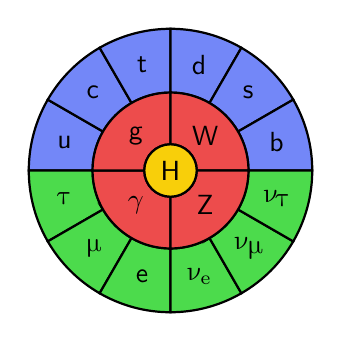
\begin{tikzpicture}[scale=0.9]
  \message{^^JSM particles}
  
  % SETTINGS
  \coordinate (O) at (0,0);
  
  % QUARKS (outer layer on top)
  \foreach \name [count=\i from 1,evaluate={\ang=int(180-\i*30)}] in {
    u,c,t,d,s,b
  }{
    \fermion[quark=\col]{\ang} %{\name}
    \node at (F-\ang) {\name};
  }
  
  % LEPTONS (outer layer on bottom)
  \foreach \name [count=\i from 0,evaluate={\ang=int(180+\i*30)}] in {
    $\PGt$,$\PGm$,e,$\PGn{\mathrm{e}}$,$\PGn{\PGm}$,$\PGn{\PGt}$
  }{
    \fermion[lepton=\col]{\ang} %{\name}
    \node at (F-\ang) {\name};
  }
  
  % GAUGE BOSONS (middle layer)
  \foreach \name [count=\i from 0,evaluate={\ang=int(180-\i*90)}] in {
    $\gamma$,g,W,Z
  }{
    \boson[gauge=\col]{\ang} %{\name}
    \node at (B-\ang) {\name};
  }
  
  % HIGGS BOSON
  \higgs
  \node at (H) {H};
  
\end{tikzpicture}
} % close foreach loop over \col


% SM PARTICLES, simple, with names
\foreach \col in {100,79}{ % change color strength
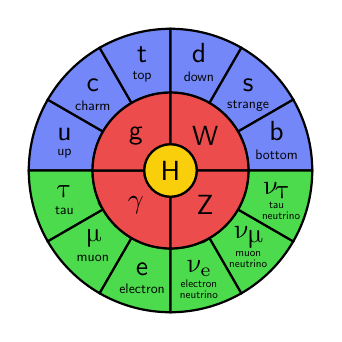
\begin{tikzpicture}[scale=0.9]
  \message{^^JSM particles}
  
  % SETTINGS
  \coordinate (O) at (0,0);
  
  % QUARKS (outer layer on top)
  \foreach \psymb/\pname [count=\i from 1,evaluate={\ang=int(180-\i*30)}] in {
    u/up,
    c/charm,
    t/top,
    d/down,
    s/strange,
    b/bottom
  }{
    \fermion[quark=\col]{\ang}
    \node[above=-3pt] at (F-\ang) {\psymb};
    \node[below=1pt,scale=0.5] at (F-\ang) {\pname};
  }
  
  % CHARGED LEPTONS (outer layer on bottom)
  \foreach \psymb/\pname [count=\i from 0,evaluate={\ang=int(180+\i*30)}] in {
    $\PGt$/tau,
    $\PGm$/muon,
    e/electron
  }{
    \fermion[lepton=\col]{\ang}
    \node[above=-3pt] at (F-\ang) {\psymb};
    \node[below=1pt,scale=0.5] at (F-\ang) {\pname};
  }
  
  % NEUTRINOS (outer layer on bottom)
  \foreach \psymb/\pname [count=\i from 0,evaluate={\ang=int(270+\i*30)}] in {
    $\PGn{\mathrm{e}}$/electron,
    $\PGn{\PGm}$/muon,
    $\PGn{\PGt}$/tau
  }{
    \fermion[lepton=\col]{\ang}
    \node[above=-3.5pt] at (F-\ang) {\psymb};
    \node[below=-0.3pt,scale=0.4,align=center] %,xshift={(\i==2)*4pt}
      at (F-\ang) {\pname\\[-2pt]\ifnum\i=2\hspace{0.8em}\fi neutrino};
  }
  
  % GAUGE BOSONS (middle layer)
  \foreach \name [count=\i from 0,evaluate={\ang=int(180-\i*90)}] in {
    $\gamma$,g,W,Z
  }{
    \boson[gauge=\col]{\ang}
    \node at (B-\ang) {\name};
  }
  
  % HIGGS BOSON
  \higgs
  \node at (H) {H};
  
\end{tikzpicture}
} % close foreach loop over \col


% SUSY PARTICLES, simple
\foreach \col in {100,79}{ % change color strength
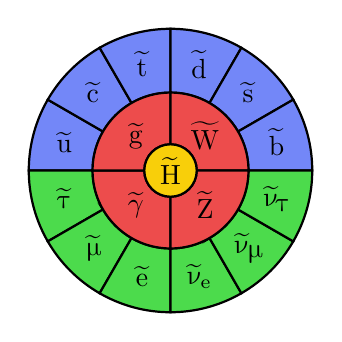
\begin{tikzpicture}[scale=0.9]
  \message{^^JSM particles}
  
  % SETTINGS
  \coordinate (O) at (0,0);
  
  % QUARKS (outer layer on top)
  \foreach \name [count=\i from 1,evaluate={\ang=int(180-\i*30)}] in {
    u,c,t,d,s,b
  }{
    \fermion[quark=\col]{\ang} %{\name}
    \node at (F-\ang) {$\mytilde{\name}$};
  }
  
  % LEPTONS (outer layer on bottom)
  \foreach \name [count=\i from 0,evaluate={\ang=int(180+\i*30)}] in {
    \widetilde{\PGt},\widetilde{\PGm},\mytilde{e},\PSGn{\mathrm{e}},\PSGn{\PGm},\PSGn{\PGt}
  }{
    \fermion[lepton=\col]{\ang} %{\name}
    \node at (F-\ang) {$\name$};
  }
  
  % GAUGE BOSONS (middle layer)
  \foreach \name [count=\i from 0,evaluate={\ang=int(180-\i*90)}] in {
    \gamma,g,W,Z
  }{
    \boson[gauge=\col]{\ang} %{\name}
    \node at (B-\ang) {$\mytilde{\name}$};
  }
  
  % HIGGS BOSON
  \higgs
  \node at (H) {$\mytilde{H}$};
  
\end{tikzpicture}
} % close foreach loop over \col


\end{document}